%!TEX program = xelatex
\documentclass[UTF8,openany,oneside]{ctexbook}
\usepackage{qau-thesis}

% 主控文件：统一组织封面、摘要、目录、正文、参考文献、附录和结尾材料。

% ===== 封面固定参数表 =====
% 在 qau-cover-info.tex 中切换学硕 / 专硕：
% 用哪个版本，就保留哪一组；另一个版本逐行加 % 注释（快捷键ctrl+T）。
% ============================================================
% 青岛农业大学毕业论文封面/英文扉页固定参数表（最终版）
% 使用方法：
% 1. 学硕：保留“学术型硕士参数”这一组；
%    同时确保“专业型硕士参数”整组前面都有 % 注释。
% 2. 专硕：取消“专业型硕士参数”整组前面的 %；
%    再把“学术型硕士参数”整组逐行加上 % 注释。
% 3. 只需要二选一，谁生效就保留谁不注释。
% ============================================================

% ===== 公共参数（中文封面 + 英文扉页） =====
% 这一组无论学硕还是专硕通常都要填写。
\classification{}
\udc{}
\secrecy{}
\schoolcode{10435}
\titleimage{assets/qau-calligraphy.jpg}
\covercity{中国·青岛}
\submityearcn{二〇二六}
\submitmonthcn{六}
\covercityen{Qingdao, China}
\submitdateen{June, 2026}
\authornameen{San Zhang}
% 英文信息建议与学校最终英文版材料保持一致。
\supervisoren{Si Li}
\secondsupervisoren{Wu Wang}
\collegeen{College of Food Science and Engineering}
\degreenameen{Master of Engineering}
\degreecategoryen{Master of Agronomy}
\professionalfielden{Food and Nutrition}

% ============================================================
% 学术型硕士参数（启用时，请取消下面整段注释，并把后面的专硕部分注释掉）
% ============================================================
%\academicmaster
%\titlecn{抗坏血酸处理对鲜切苹果褐变抑制效果及品质保持机制的研究}
%\titleen{Study on the Effect of Ascorbic Acid Treatment on Browning Inhibition and Quality Maintenance Mechanisms in Fresh-Cut Apples}
%\authorname{张三}
%\supervisor{李四\quad 教授}
%\major{食品科学与工程}
%\direction{果蔬贮藏与加工}

% ============================================================
% 专业型硕士参数（当前默认启用）
% 二选一：当前仓库默认启用专硕示例，提交前请按本人学位类型核对。
% ============================================================
\professionalmaster
\titlecn{抗坏血酸处理对鲜切苹果褐变抑制效果及品质保持机制的研究}
\titleen{Study on the Effect of Ascorbic Acid Treatment on Browning Inhibition and Quality Maintenance Mechanisms in Fresh-Cut Apples}
\authorname{张三}
\supervisor{李四\quad 教授}
\secondsupervisor{王五\quad 高级工程师}
\degreecategory{农业硕士}
\professionalfield{食品与营养}


\graphicspath{{figures/}{assets/}}
% 图片默认搜索路径：正文插图放 figures/，封面字样等资源放 assets/。

\begin{document}

% ===== 封面与前置部分 =====
\pagestyle{empty}
\thispagestyle{empty}

\begingroup
\centering
\setlength{\tabcolsep}{0pt}
\setlength{\parindent}{0pt}

% ===== 顶部元数据 =====
\begin{minipage}[t]{0.42\textwidth}
  \raggedright
   {\songti\zihao{4}\makebox[3em][s]{分类号}\QAUcoverline[3cm]{\qauclassification}\par}
   \vspace{0.72cm}
   {{\qauTimes\zihao{4}\makebox[3em][s]{U\hfill D\hfill C}}\QAUcoverlineTimes[3cm]{\qauudc}\par}
\end{minipage}
\hfill
\begin{minipage}[t]{0.31\textwidth}
  \raggedright
  {\songti\zihao{4}\makebox[4em][s]{密级}\QAUcoverline[3cm]{\qausecrecy}\par}
  \vspace{0.82cm}
  {\songti\zihao{4}\makebox[4em][s]{单位代码}\QAUcoverlineTimes[3cm]{\qauschoolcode}\par}
\end{minipage}

\vspace*{1.80cm}

% ===== 校名字样 =====
\includegraphics[width=0.4\textwidth]{\qautitleimage}

\vspace{0.78cm}

% ===== 论文类型 =====
\ifthenelse{\equal{\qaucoverstyle}{professional}}
    {\QAUcovertitleprofessional\par}
        {\QAUcovertitleacademic\par}

\vspace{1.02cm}

% ===== 中文题目 =====
{\songti\zihao{-2}
\begin{minipage}{0.84\textwidth}
  \centering
  \setlength{\baselineskip}{30bp}
  \qautitle
\end{minipage}\par}

\vspace{0.60cm}

% ===== 英文题目 =====
{{\qauTimes\fontsize{18bp}{20bp}\selectfont
\begin{minipage}{0.85\textwidth}
  \centering
  \qauetitle
\end{minipage}\par}}

\ifthenelse{\equal{\qaucoverstyle}{professional}}{\vspace{0.78cm}}{\vspace{0.92cm}}

% ===== 作者信息 =====
\renewcommand{\arraystretch}{1.68}
\ifthenelse{\equal{\qaucoverstyle}{professional}}{
  {\zihao{4}
  \begin{tabular}{@{}p{2.55cm}@{}p{5.85cm}@{}}
    {\QAUlabelstyle{姓\hspace{1.6em}名：}} & \QAUcoverlineKai[5.7cm]{\qauauthor} \\
    {\QAUlabelstyle{指导教师：}} & \QAUcoverlineKai[5.7cm]{\qausupervisor} \\
    {\QAUlabelstyle{第二导师：}} & \QAUcoverlineKai[5.7cm]{\qausecondsupervisor} \\
    {\QAUlabelstyle{学位类别：}} & \QAUcoverlineKai[5.7cm]{\qaudegreecategory} \\
    {\QAUlabelstyle{专业领域：}} & \QAUcoverlineKai[5.7cm]{\qauprofessionalfield} \\
  \end{tabular}\par}
}{
  {\zihao{4}
  \begin{tabular}{@{}p{2.55cm}@{}p{5.85cm}@{}}
    {\QAUlabelstyle{姓\hspace{1.6em}名：}} & \QAUcoverlineKai[5.7cm]{\qauauthor} \\
    {\QAUlabelstyle{指导教师：}} & \QAUcoverlineKai[5.7cm]{\qausupervisor} \\
    {\QAUlabelstyle{学科专业：}} & \QAUcoverlineKai[5.7cm]{\qaumajor} \\
    {\QAUlabelstyle{研究方向：}} & \QAUcoverlineKai[5.7cm]{\qaudirection} \\
  \end{tabular}\par}
}

\vfill

{\kaishu\zihao{4}\qaucity\par}
\vspace{0.20cm}
{\kaishu\zihao{4}\qaudate\par}

\endgroup
\clearpage

\clearpage
\thispagestyle{empty}

\begingroup
\centering
\setlength{\parindent}{0pt}

\ifthenelse{\equal{\qaucoverstyle}{professional}}{%
  \vspace*{0.1cm}
  {\qauCorsiva\fontsize{32bp}{28bp}\selectfont Qingdao Agricultural University\par}
  \vspace{0.48cm}
  {{\qauTimes\fontsize{22bp}{24bp}\selectfont The Thesis of Professional Master\par}}

  \vspace{3.15cm}

  {{\qauTimes\fontsize{20bp}{24bp}\selectfont
  \begin{minipage}{0.9\textwidth}
    \centering
    \setlength{\baselineskip}{24bp}
    \qauetitle
  \end{minipage}\par}}

  \vspace{1.35cm}
  {{\qauTimes\fontsize{16bp}{20bp}\selectfont Graduate with Professional Master Degree:\par}}

  \vspace{1.95cm}
  {{\qauTimes\bfseries\fontsize{16bp}{20bp}\selectfont \qauauthoren\par}}

  \vspace{1.45cm}
  {{\qauTimes\fontsize{15bp}{19bp}\selectfont Mentor: \qausupervisoren\par}}
  \QAUifemptyTF{\qausecondsupervisoren}{}{%
    \vspace{0.42cm}
    {{\qauTimes\fontsize{15bp}{19bp}\selectfont Second Mentor: \qausecondsupervisoren\par}}}

  \vspace{1.65cm}
  {{\qauTimes\fontsize{15bp}{19bp}\selectfont Type of Professional Degree:\ \textbf{\qaudegreecategoryen}\par}}
  \vspace{0.42cm}
  {{\qauTimes\fontsize{15bp}{19bp}\selectfont Academic field:\ \textbf{\qauprofessionalfielden}\par}}

  \vfill
  {{\qauTimes\fontsize{13bp}{16bp}\selectfont \qaucityen\par}}
  \vspace{0.15cm}
  {{\qauTimes\fontsize{13bp}{16bp}\selectfont \qaudateen\par}}
}{%
  \vspace*{1.55cm}
  {{\qauTimes\bfseries\fontsize{24bp}{31bp}\selectfont
  \begin{minipage}{0.88\textwidth}
    \centering
    \setlength{\baselineskip}{31bp}
    \qauetitle
  \end{minipage}\par}}

  \vspace{0.95cm}
  {{\qauTimes\fontsize{16bp}{20bp}\selectfont Thesis submitted to\par}}

  \vspace{0.92cm}
  {{\qauTimes\fontsize{23bp}{27bp}\selectfont Qingdao Agricultural University\par}}

  \vspace{1.35cm}
  {{\qauTimes\fontsize{16bp}{20bp}\selectfont In Fulfillment of the Requirement\par}}

  \vspace{0.72cm}
  {{\qauTimes\bfseries\fontsize{16bp}{19bp}\selectfont for the Degree of\par}}

  \vspace{0.88cm}
  {{\qauTimes\bfseries\fontsize{21bp}{25bp}\selectfont \qaudegreeen\par}}

  \vspace{0.95cm}
  {{\qauTimes\bfseries\fontsize{16bp}{20bp}\selectfont \qauauthoren\par}}

  \vspace{1.00cm}
  {{\qauTimes\bfseries\fontsize{15bp}{19bp}\selectfont (\qaucollegeen)\par}}

  \vspace{0.88cm}
  {{\qauTimes\bfseries\fontsize{15bp}{19bp}\selectfont Supervisor: \qausupervisoren\par}}

  \vfill
  {{\qauTimes\fontsize{13bp}{16bp}\selectfont \qaucityen\par}}
  \vspace{0.15cm}
  {{\qauTimes\fontsize{13bp}{16bp}\selectfont \qaudateen\par}}
}



\endgroup
\clearpage

\clearpage
\thispagestyle{empty}
\begingroup
\setlength{\parindent}{2em}
\setstretch{1.50}

%\vspace*{2.4cm}

\begin{center}
{\heiti\zihao{2}独\quad 创\quad 性\quad 声\quad 明\par}
\end{center}

\vspace{0.95cm}

{\songti\zihao{-4}
本人声明所呈交的论文是我个人在导师指导下进行的研究工作及取得的研究成果。尽我所知，除了文中特别加以标注和致谢的地方外，论文中不包含其他人已经发表或撰写过的研究成果，也不包含为获得青岛农业大学或其他教育机构的学位或证书而使用过的材料。与我一同工作的人员对本研究所做的任何贡献均已在论文中作了明确的说明并表示了谢意。\par}

\vspace{1.8cm}

{\songti\zihao{-4}研究生签名：\hspace{5.0cm}时间：\hspace{1.1cm}年\hspace{0.9cm}月\hspace{0.9cm}日}

\vspace{2.35cm}

\begin{center}
{\heiti\zihao{2}关于论文使用授权的说明\par}
\end{center}

\vspace{0.72cm}

{\songti\zihao{-4}
本人完全了解青岛农业大学有关保留、使用学位论文的规定，即：学校有权保留送交论文的复印件和磁盘，允许论文被查阅和借阅，可以采用影印、缩印或扫描等复制手段保存、汇编学位论文。同意青岛农业大学可以用不同方式在不同媒体上发表、传播学位论文的全部或部分内容。

\textbf{（保密的学位论文在解密后应遵守此协议）}\par}

\vspace{1.5cm}

{\songti\zihao{-4}研究生签名：\hspace{5cm}时间：\hspace{1.1cm}年\hspace{0.9cm}月\hspace{0.9cm}日}

\endgroup
\thispagestyle{empty}
\vspace*{0.5cm}
{\songti\zihao{-4}导师签名：\hspace{5.4cm}时间：\hspace{1.1cm}年\hspace{0.9cm}月\hspace{0.9cm}日}

\clearpage

\pagenumbering{Roman}
\setcounter{page}{1}
\pagestyle{qaufront}
\QAUabstracttitleCN

{\kaishu\fontsize{12bp}{21bp}\selectfont
摘要（中文）语言应力求简明精炼，硕士论文摘要不超过1000个汉字；摘要内容应能反映学位论文的主要信息（包括研究的背景和目的、研究方法及过程、结果和结论、研究的意义等），不读论文全文也能获取必要信息，即摘要应具有独立性和自含性；摘要不能与前言相互混淆；摘要应避免使用图、表、化学结构式、非公知公用的符号和术语。\par}

\vspace{0.5\baselineskip}

{\kaishu\fontsize{12bp}{21bp}\selectfont
\noindent\hspace*{2em}{\heiti\zihao{-4}关键词：}{\kaishu\zihao{-4}鲜切苹果；抗坏血酸；褐变抑制；品质保持；学位论文模板}\par}

\clearpage
\QAUabstracttitleEN

{\qauTimes\fontsize{10.5bp}{15.75bp}\selectfont
The abstract should be concise and refined. For a master's thesis, the Chinese abstract should normally contain no more than 1,000 Chinese characters. It should reflect the major information of the thesis, including the research background and objective, methods and procedures, results and conclusions, as well as the academic or practical significance of the study. The abstract should be independent and self-contained so that readers can obtain the necessary information without reading the full thesis. It should not be confused with the introduction, and figures, tables, chemical structural formulas, or symbols and terms that are not generally known should be avoided.\par}

\vspace{0.5\baselineskip}

{\qauTimes\fontsize{10.5bp}{15.75bp}\selectfont
\noindent\hspace*{2em}{\bfseries Keywords: }Fresh-cut apple; Ascorbic acid; Browning inhibition; Quality maintenance; Thesis template\par}

\clearpage
% 中文目录为手动样式命令，便于精确控制目录页标题与条目间距。
\QAUmanualtoc
\clearpage
\QAUmanualtoce

\QAUentocchapter{Chapter 1\quad Introduction}{chap:intro}
\QAUentocsection{1.1\quad Research Background}{sec:intro-background}
\QAUentocsubsection{1.1.1\quad Current Status of Fresh-cut Browning Research}{subsec:intro-status}
\QAUentocsection{1.2\quad Literature Review}{sec:intro-review}
\QAUentocsubsection{1.2.1\quad Research Progress in Browning Inhibition}{subsec:intro-progress}
\QAUentocsection{1.3\quad Significance and Research Contents}{sec:intro-significance-content}
\QAUentocsubsection{1.3.1\quad Significance of the Study}{subsec:intro-significance}
\QAUentocsubsection{1.3.2\quad Research Contents}{subsec:intro-contents}
\QAUentocsection{1.4\quad Research Route}{sec:intro-route}

\QAUentocchapter{Chapter 2\quad Effect of XXX on XXXX}{chap:ch2}
\QAUentocsection{2.1\quad Materials and Methods}{sec:ch2-methods}
\QAUentocsubsection{2.1.1\quad Materials and Reagents}{subsec:ch2-materials}
\QAUentocsubsection{2.1.2\quad Instruments and Equipment}{subsec:ch2-instruments}
\QAUentocsubsection{2.1.3\quad Preparation of XXXX}{subsec:ch2-preparation}
\QAUentocsubsection{2.1.4\quad Determination of XXXX}{subsec:ch2-determination}
\QAUentocsubsection{2.1.5\quad Statistical Analysis}{subsec:ch2-statistics}
\QAUentocsection{2.2\quad Results and Discussion}{sec:ch2-results}
\QAUentocsubsection{2.2.1\quad XXXXXXXXX}{subsec:ch2-result-a}
\QAUentocsubsection{2.2.2\quad XXXXXXXXX}{subsec:ch2-result-b}
\QAUentocsection{2.3\quad Summary}{sec:ch2-summary}

\QAUentocchapter{Chapter 3\quad Effect of XXX on XXXX}{chap:ch3}
\QAUentocsection{3.1\quad Materials and Methods}{sec:ch3-methods}
\QAUentocsubsection{3.1.1\quad Materials and Reagents}{subsec:ch3-materials}
\QAUentocsubsection{3.1.2\quad Instruments and Equipment}{subsec:ch3-instruments}
\QAUentocsubsection{3.1.3\quad Preparation of XXXX}{subsec:ch3-preparation}
\QAUentocsubsection{3.1.4\quad Determination of XXXX}{subsec:ch3-determination}
\QAUentocsubsection{3.1.5\quad Statistical Analysis}{subsec:ch3-statistics}
\QAUentocsection{3.2\quad Results and Discussion}{sec:ch3-results}
\QAUentocsubsection{3.2.1\quad XXXXXXXXX}{subsec:ch3-result-a}
\QAUentocsection{3.3\quad Summary}{sec:ch3-summary}

\QAUentocchapter{Chapter 4\quad Effect of XXX on XXXX}{chap:ch4}
\QAUentocsection{4.1\quad Materials and Methods}{sec:ch4-methods}
\QAUentocsubsection{4.1.1\quad Materials and Reagents}{subsec:ch4-materials}
\QAUentocsubsection{4.1.2\quad Instruments and Equipment}{subsec:ch4-instruments}
\QAUentocsubsection{4.1.3\quad Preparation of XXXX}{subsec:ch4-preparation}
\QAUentocsubsection{4.1.4\quad Determination of XXXX}{subsec:ch4-determination}
\QAUentocsubsection{4.1.5\quad Statistical Analysis}{subsec:ch4-statistics}
\QAUentocsection{4.2\quad Results and Discussion}{sec:ch4-results}
\QAUentocsubsection{4.2.1\quad XXXXXXXXX}{subsec:ch4-result-a}
\QAUentocsection{4.3\quad Summary}{sec:ch4-summary}

\QAUentocchapter{Chapter 5\quad Effect of XXX on XXXX}{chap:ch5}
\QAUentocsection{5.1\quad Materials and Methods}{sec:ch5-methods}
\QAUentocsubsection{5.1.1\quad Materials and Reagents}{subsec:ch5-materials}
\QAUentocsubsection{5.1.2\quad Instruments and Equipment}{subsec:ch5-instruments}
\QAUentocsubsection{5.1.3\quad Preparation of XXXX}{subsec:ch5-preparation}
\QAUentocsubsection{5.1.4\quad Determination of XXXX}{subsec:ch5-determination}
\QAUentocsubsection{5.1.5\quad Statistical Analysis}{subsec:ch5-statistics}
\QAUentocsection{5.2\quad Results and Discussion}{sec:ch5-results}
\QAUentocsubsection{5.2.1\quad XXXXXXXXX}{subsec:ch5-result-a}
\QAUentocsection{5.3\quad Summary}{sec:ch5-summary}

\QAUentocchapter{Conclusion and Prospects}{chap:conclusion}
\QAUentocchapter{References}{chap:references}
\QAUentocchapter{Appendix A\quad Supplementary Experimental Data and Notes}{app:appendixA}
\QAUentocchapter{Appendix B\quad Supplementary Figures and Statistical Analyses}{app:appendixB}
\QAUentocchapter{Supervisor Group Opinion}{chap:opinion}
\QAUentocchapter{Acknowledgements}{chap:acknowledgements}
\QAUentocchapter{Biography}{chap:resume}
\QAUentocchapter{Academic Achievements During Degree Study}{chap:achievements}

\clearpage

% ===== 主体部分 =====
\pagestyle{qau}
\pagenumbering{arabic}
\setcounter{page}{1}
\chapter{绪论}\label{chap:intro}

鲜切苹果因食用便捷、营养价值较高而受到广泛欢迎\citep{Arnold2022CRFSFS}，但切割损伤会诱发局部氧化应激与酶促褐变反应，进而导致色泽劣变、风味下降及货架期缩短\citep{Fan2023CRFSN}。围绕鲜切苹果褐变形成、护色剂作用位置以及品质保持机制开展系统研究，对于鲜切果蔬精准护色与品质调控具有重要意义。

\section{苹果XXX}\label{sec:intro-background}

鲜切苹果在加工、贮运与销售过程中易发生褐变，其本质与切割损伤后酚类底物、多酚氧化酶、氧气以及细胞结构破坏之间的耦合作用密切相关\citep{Sui2023EBC,Zeng2025FoodControl,Liu2025CRFSFS}。

\subsection{苹果XXX}\label{subsec:intro-status}

目前关于鲜切苹果褐变的研究已从整体品质评价逐步拓展到组织结构等方面。目前关于鲜切苹果褐变的研究已从整体品质评价逐步拓展到组织结构等方面。目前关于鲜切苹果褐变的研究已从整体品质评价逐步拓展到组织结构等方面。

\section{苹果XXX}\label{sec:intro-review}

现有文献多围绕抗坏血酸、柠檬酸、钙盐等护色剂的应用展开，并结合综合色差、褐变指数、酶活性变化和营养保持水平评价处理效果。现有文献多围绕抗坏血酸、柠檬酸、钙盐等护色剂的应用展开，并结合综合色差、褐变指数、酶活性变化和营养保持水平评价处理效果。

\subsection{苹果XXX}\label{subsec:intro-progress}

在褐变抑制方面，研究重点已由单纯的工艺经验优化逐渐转向机制解释。在褐变抑制方面，研究重点已由单纯的工艺经验优化逐渐转向机制解释。在褐变抑制方面，研究重点已由单纯的工艺经验优化逐渐转向机制解释。

\section{研究意义与内容}\label{sec:intro-significance-content}

本研究以鲜切苹果为对象，拟从XXX等角度，构建鲜切苹果褐变抑制与品质保持机制的研究框架。

\subsection{研究意义}\label{subsec:intro-significance}

通过明确抗坏血酸在鲜切苹果组织中的XXXX，可为鲜切果蔬护色技术的精准调控提供理论依据，并为后续开发高效护色工艺和评价体系提供参考。

\subsection{研究内容}\label{subsec:intro-contents}

研究内容主要包括：鲜切苹果褐变XXXX；外源抗坏血酸XXXX；典型处理条件下品质保持效果评价；以及基于XXXX的褐变抑制机制解析。

\section{研究路线}\label{sec:intro-route}

%本节用于放置论文技术路线图或研究思路图，后续可根据课题需要替换为正式图片。

\begin{center}
	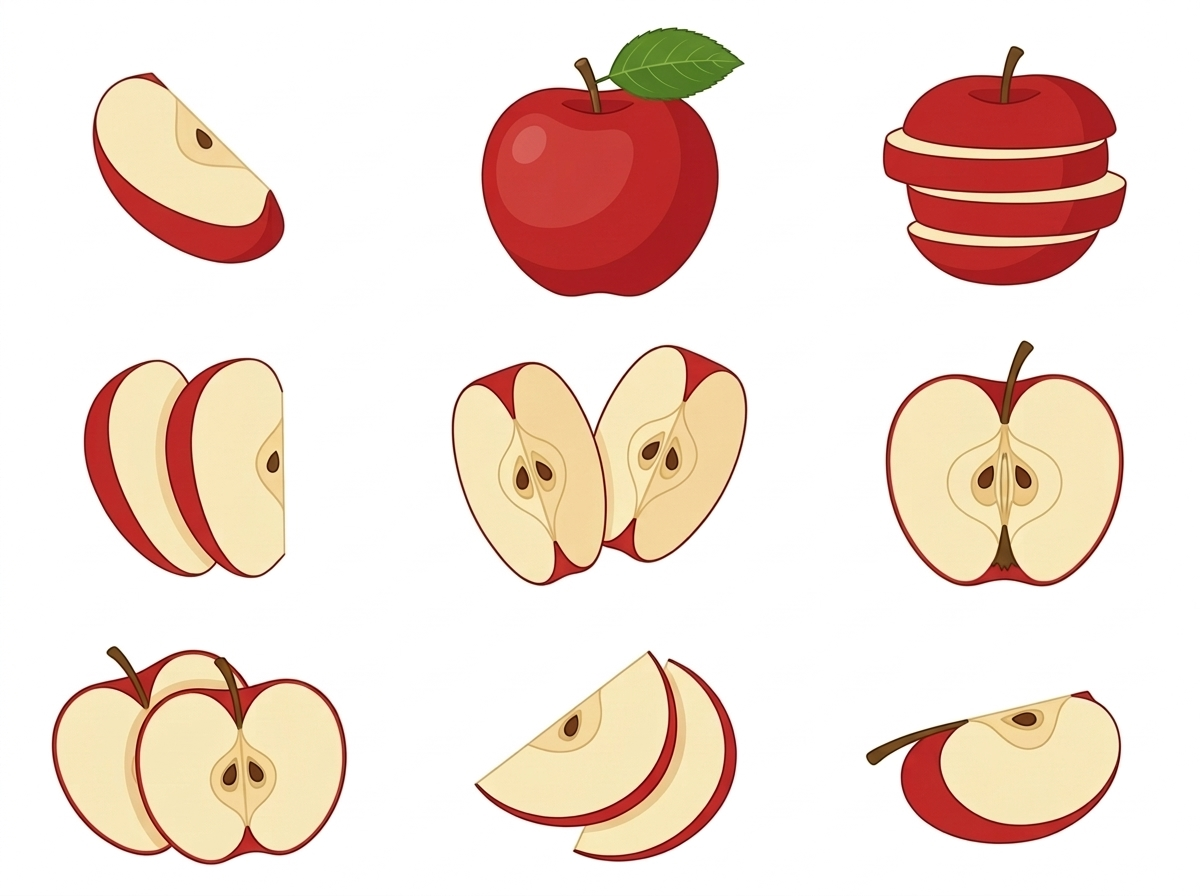
\includegraphics[width=0.6\textwidth]{figures/apple.png}
	\captionof{figure}[研究路线]{研究路线\par
		{\qauTimes\fontsize{10.5bp}{15.75bp}\selectfont \textbf{Fig.~\thefigure\ Research route}}}
	\label{fig:research-route}
\end{center}
\chapter{XXX对XXXX的影响}\label{chap:ch2}

本段为章前导语，主要用于对本章研究内容进行简要引入与概括说明。通常可包括本章研究目的、主要研究内容、拟解决的问题以及章节结构安排等，以增强章节之间的衔接性和整体逻辑性。

\section{材料与方法}\label{sec:ch2-methods}

\subsection{材料与试剂}\label{subsec:ch2-materials}

本节用于填写试验原料来源、主要化学试剂名称、纯度等级、生产厂家及批次信息等。

\subsection{仪器与设备}\label{subsec:ch2-instruments}

本节用于填写主要实验仪器、型号、生产厂家及关键测试设备信息。

\subsection{XXXX的制备}\label{subsec:ch2-preparation}

本节用于描述样品制备、处理条件设置及工艺流程。

\subsection{XXXX的测定}\label{subsec:ch2-determination}

本节用于描述指标测定方法、计算公式和操作要点。

例如，综合指标的计算过程可写为：
\begin{align}
	Z_i &= \sum_{j=1}^{n}\omega_j z_{ij} \\
	z_{ij} &= \frac{x_{ij}-\bar{x}_j}{s_j} \\
	s_j &= \sqrt{\frac{1}{m-1}\sum_{i=1}^{m}\left(x_{ij}-\bar{x}_j\right)^2}
	\label{eq:ch2-example}
\end{align}

式中，$Z_i$ 表示第 $i$ 个样品的综合得分；$\omega_j$ 表示第 $j$ 个指标的权重；$z_{ij}$ 表示标准化后的指标值；$\bar{x}_j$ 表示第 $j$ 个指标的平均值；$s_j$ 表示标准差。

\subsection{统计与分析}\label{subsec:ch2-statistics}

本节用于说明试验重复次数、统计方法与绘图软件等。

\section{结果与讨论}\label{sec:ch2-results}

\subsection{XXXXXXXXX}\label{subsec:ch2-result-a}

本部分用于展示研究结果，并结合相关理论与文献对结果进行分析讨论，阐明其变化规律、影响因素及可能作用机制。涉及上下标、公式、变量符号及统计学表达时，建议采用规范的 \LaTeX{} 数学格式书写，如$\mathrm{O}_2^{\cdot-}$、$k_{\mathrm{cat}}$、$R^2$、$p<0.05$、$\Delta E$、$\mu\mathrm{m}$、$10^{-3}$、$a_i^{(n)}$、$\mathrm{PPO}_{\mathrm{activity}}$等。

\begin{center}
	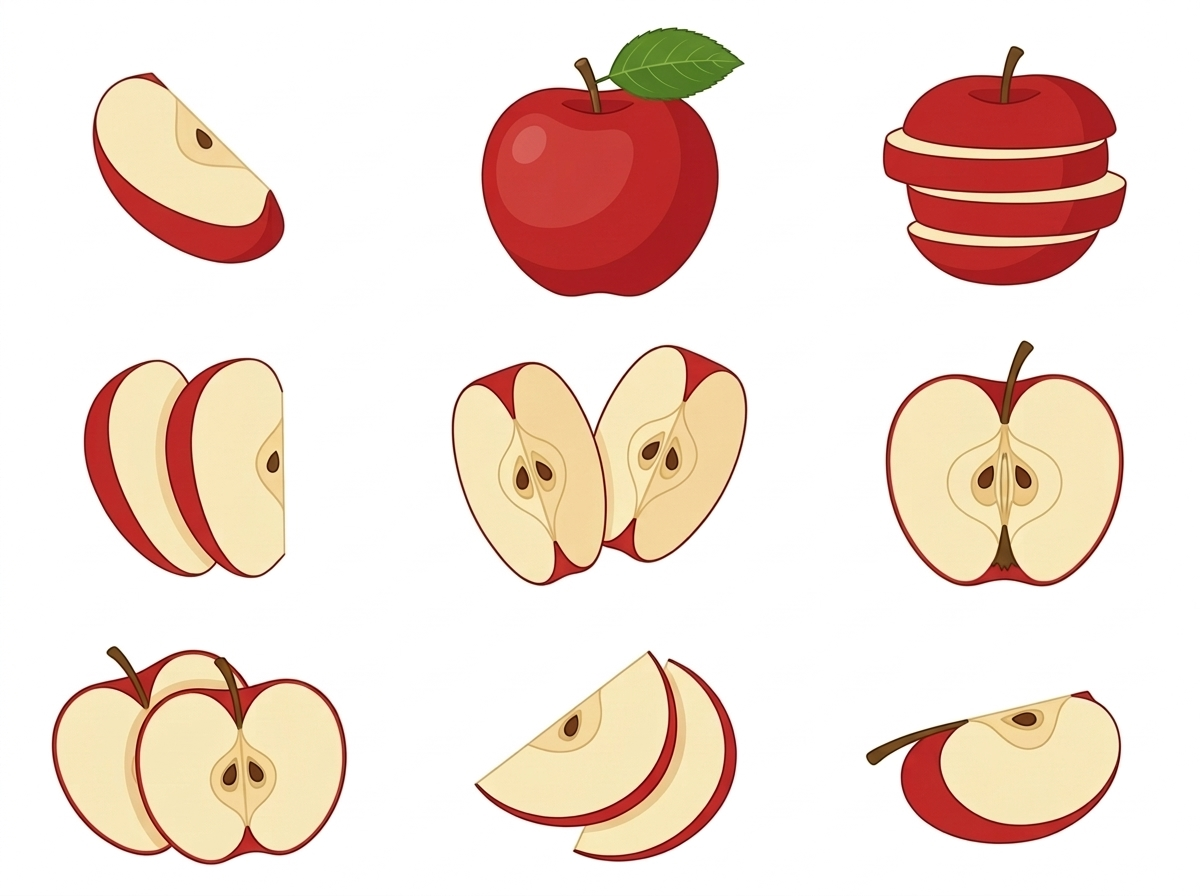
\includegraphics[width=0.6\textwidth]{figures/apple.png}
	\captionof{figure}[XXXX变化趋势]{XXXX变化趋势。\par
		（A）XXXX；（B）XXXX；（C）XXXX。\par
		注：不同小写字母代表存在显著差异（$p<0.05$）。\par
		{\qauTimes\fontsize{10.5bp}{15.75bp}\selectfont \textbf{Fig.~\thefigure\ Trend of XXXX changes.}}\par
		{\qauTimes\fontsize{10.5bp}{15.75bp}\selectfont \textbf{(A) XXXX; (B) XXXX; (C) XXXX.}}\par
        {\qauTimes\fontsize{10.5bp}{15.75bp}\selectfont \textbf{Different lowercase letters indicate significant differences (\boldmath$p<0.05$).}}}
	\label{fig:ch2-example}
\end{center}

\subsection{XXXXXXXXX}\label{subsec:ch2-result-b}

本部分用于展示研究结果，并结合相关理论与文献对结果进行分析讨论，阐明其变化规律、影响因素及可能作用机制。涉及上下标、公式、变量符号及统计学表达时，建议采用规范的 \LaTeX{} 数学格式书写，如$\mathrm{O}_2^{\cdot-}$、$k_{\mathrm{cat}}$、$R^2$、$p<0.05$、$\Delta E$、$\mu\mathrm{m}$、$10^{-3}$、$a_i^{(n)}$、$\mathrm{PPO}_{\mathrm{activity}}$等。

\begin{center}
	\captionof{table}[示例表题：不同处理下指标测定结果]{不同处理下指标测定结果\par
		{\qauTimes\fontsize{10.5bp}{15.75bp}\selectfont \textbf{Table~\thetable\ Determination results of different indices under different treatments}}}
	\label{tab:ch2-example}
	\renewcommand{\arraystretch}{1.5}
	{\songti\zihao{5}
		\begin{tabular*}{0.85\textwidth}{@{\extracolsep{\fill}}>{\centering\arraybackslash}m{0.18\textwidth}>{\centering\arraybackslash}m{0.26\textwidth}>{\centering\arraybackslash}m{0.26\textwidth}}
			\toprule
			处理 & 指标 1 & 指标 2 \\
			\midrule
			CK & 0.00$\pm$0.00\textsuperscript{a} & 0.00$\pm$0.00\textsuperscript{a} \\
			T1 & 0.00$\pm$0.00\textsuperscript{b} & 0.00$\pm$0.00\textsuperscript{ab} \\
			T2 & 0.00$\pm$0.00\textsuperscript{c} & 0.00$\pm$0.00\textsuperscript{b} \\
			\bottomrule
		\end{tabular*}
		\par
		{\center 注：不同小写字母代表存在显著差异（$p<0.05$）。\par}
	}
\end{center}

\section{小结}\label{sec:ch2-summary}

本节用于归纳本章主要结果，概括关键发现并为下一章研究奠定基础。

\input{chapters/03-chapter-three}
\chapter{XXX对XXXX的影响}\label{chap:ch4}

本段为章前导语，主要用于对本章研究内容进行简要引入与概括说明。通常可包括本章研究目的、主要研究内容、拟解决的问题以及章节结构安排等，以增强章节之间的衔接性和整体逻辑性。

\section{材料与方法}\label{sec:ch4-methods}

\subsection{材料与试剂}\label{subsec:ch4-materials}

本节用于填写试验原料来源、主要化学试剂名称、纯度等级、生产厂家及批次信息等。

\subsection{仪器与设备}\label{subsec:ch4-instruments}

本节用于填写主要实验仪器、型号、生产厂家及关键测试设备信息。

\subsection{XXXX的制备}\label{subsec:ch4-preparation}

本节用于描述样品制备、处理条件设置及工艺流程。

\subsection{XXXX的测定}\label{subsec:ch4-determination}

本节用于描述指标测定方法、计算公式和操作要点。

\subsection{统计与分析}\label{subsec:ch4-statistics}

统计与分析方法同 \ref{subsec:ch2-statistics} 节，如有特殊情况另作说明。

\section{结果与讨论}\label{sec:ch4-results}

\subsection{XXXXXXXXX}\label{subsec:ch4-result-a}

本部分用于展示研究结果，并结合相关理论与文献对结果进行分析讨论，阐明其变化规律、影响因素及可能作用机制。涉及上下标、公式、变量符号及统计学表达时，建议采用规范的 \LaTeX{} 数学格式书写，如$\mathrm{O}_2^{\cdot-}$、$k_{\mathrm{cat}}$、$R^2$、$p<0.05$、$\Delta E$、$\mu\mathrm{m}$、$10^{-3}$、$a_i^{(n)}$、$\mathrm{PPO}_{\mathrm{activity}}$等。

\section{小结}\label{sec:ch4-summary}

本节用于归纳本章主要结果，概括关键发现并为下一章研究奠定基础。
\input{chapters/05-chapter-five}
\QAUchapterstar{结论与展望}\label{chap:conclusion}

{\kaishu\fontsize{14bp}{28bp}\selectfont 6.1\quad 主要结论\par}
\vspace{7pt}
本文在模板示例中用于展示“结论与展望”部分的写法。正式撰写时，可在此归纳全文的核心发现、创新点以及理论或应用价值。

{\kaishu\fontsize{14bp}{28bp}\selectfont 6.2\quad 展望\par}
\vspace{7pt}
本节用于概述尚待解决的问题、后续研究方向以及课题深化路径等内容。
% 如需增删章节，直接在此处调整 input 顺序即可。

% ===== 参考文献 =====
\clearpage
\phantomsection\label{chap:references}
% 当前默认采用“著者-年份制”参考文献样式；如需顺序编码制，可改为 gbt7714-qau。
\bibliographystyle{gbt7714-qau-ay}
\bibliography{ref}

% ===== 结尾部分 =====
\QAUappendixsetup
\chapter{补充试验数据与说明}\label{app:appendixA}

本附录用于放置不便纳入正文、但对理解研究过程与结果具有辅助价值的补充材料，例如原始测定项目列表、补充图表、参数设定说明、缩略语说明及统计分析补充结果等。附录内容的编排原则应与正文保持一致，文字说明采用宋体小四，图题表题格式与正文相同。

\section{缩略语说明示例}

\begin{center}
	\captionof{table}[研究中常用缩略语示例]{研究中常用缩略语示例\par
		{\qauTimes\fontsize{10.5bp}{15.75bp}\selectfont \textbf{Table~\thetable\ Examples of common abbreviations used in this study}}}
	\label{tab:appendix-abbr}
	\renewcommand{\arraystretch}{1.5}
	{\songti\zihao{5}
		\begin{tabular*}{0.8\textwidth}{@{\extracolsep{\fill}}>{\centering\arraybackslash}m{0.20\textwidth}>{\centering\arraybackslash}m{0.50\textwidth}}
			\toprule
			缩略语 & 含义 \\
			\midrule
			AA & 抗坏血酸 (Ascorbic acid) \\
			BI & 褐变指数 (Browning index) \\
			PPO & 多酚氧化酶 (Polyphenol oxidase) \\
			POD & 过氧化物酶 (Peroxidase) \\
			\bottomrule
		\end{tabular*}
	}
\end{center}

\section{补充图表示例}

\begin{center}
	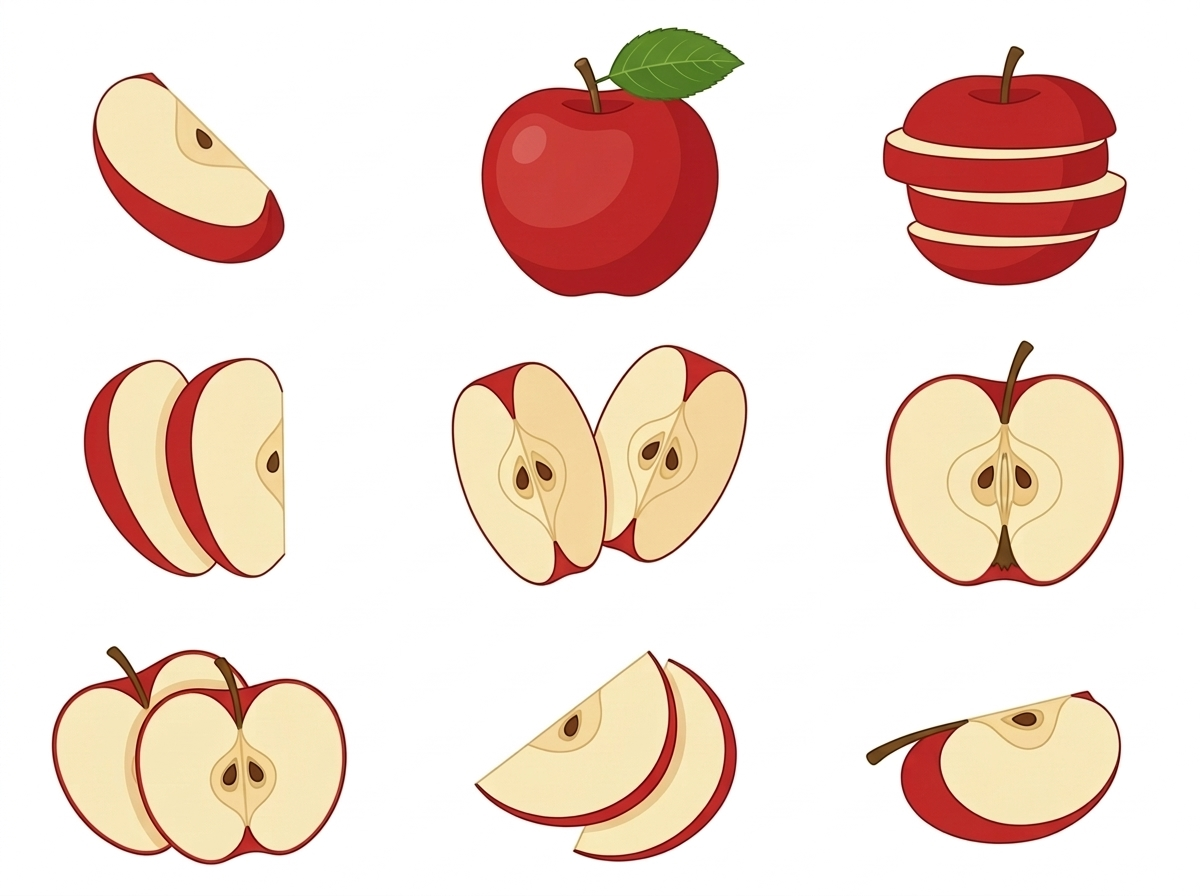
\includegraphics[width=0.45\textwidth]{figures/apple.png}
    \captionof{figure}[附录 A 中补充图片占位示例]{附录 A 中补充图片占位示例。\par
	（A）XXXX；（B）XXXX；（C）XXXX。\par
	注：不同小写字母代表存在显著差异（$p<0.05$）。\par
	{\qauTimes\fontsize{10.5bp}{15.75bp}\selectfont \textbf{Fig.~\thefigure\ Example of supplementary figure in Appendix B.}}\par
	{\qauTimes\fontsize{10.5bp}{15.75bp}\selectfont \textbf{(A) XXXX; (B) XXXX; (C) XXXX.}}\par
    {\qauTimes\fontsize{10.5bp}{15.75bp}\selectfont \textbf{Different lowercase letters indicate significant differences (\boldmath$p<0.05$).}}}
	\label{fig:appendix-layer}
\end{center}

附录中的图表仍建议按照所在附录章节顺序连续编号，并在正文中首次引用相关附录时给出明确指引，例如“详见附录 A 中表 A.1”。
\chapter{补充图表与统计分析示例}\label{app:appendixB}

本附录用于展示第二类补充材料的排版方式，例如额外统计结果、模型参数说明、补充流程图及原始图片等。附录 B 与附录 A 的图表编号独立连续，并保持与正文一致的题注样式。

\section{补充表格示例}

\begin{center}
	\captionof{table}[附录 B 中补充统计结果示例]{附录 B 中补充统计结果示例\par
		{\qauTimes\fontsize{10.5bp}{15.75bp}\selectfont \textbf{Table~\thetable\ Example of supplementary statistical results in Appendix B}}}
	\label{tab:appendix-b-stat}
	\renewcommand{\arraystretch}{1.5}
	{\songti\zihao{5}
		\begin{tabular*}{0.8\textwidth}{@{\extracolsep{\fill}}>{\centering\arraybackslash}m{0.18\textwidth}>{\centering\arraybackslash}m{0.26\textwidth}>{\centering\arraybackslash}m{0.26\textwidth}}
			\toprule
			{\songti\zihao{5}处理} & {\songti\zihao{5}指标 1} & {\songti\zihao{5}指标 2} \\
			\midrule
			CK & 0.00$\pm$0.00\textsuperscript{a} & 0.00$\pm$0.00\textsuperscript{a} \\
			T1 & 0.00$\pm$0.00\textsuperscript{b} & 0.00$\pm$0.00\textsuperscript{ab} \\
			T2 & 0.00$\pm$0.00\textsuperscript{c} & 0.00$\pm$0.00\textsuperscript{b} \\
			\bottomrule
		\end{tabular*}
	}
\end{center}

%\newpage

\section{补充图片示例}

\begin{center}
	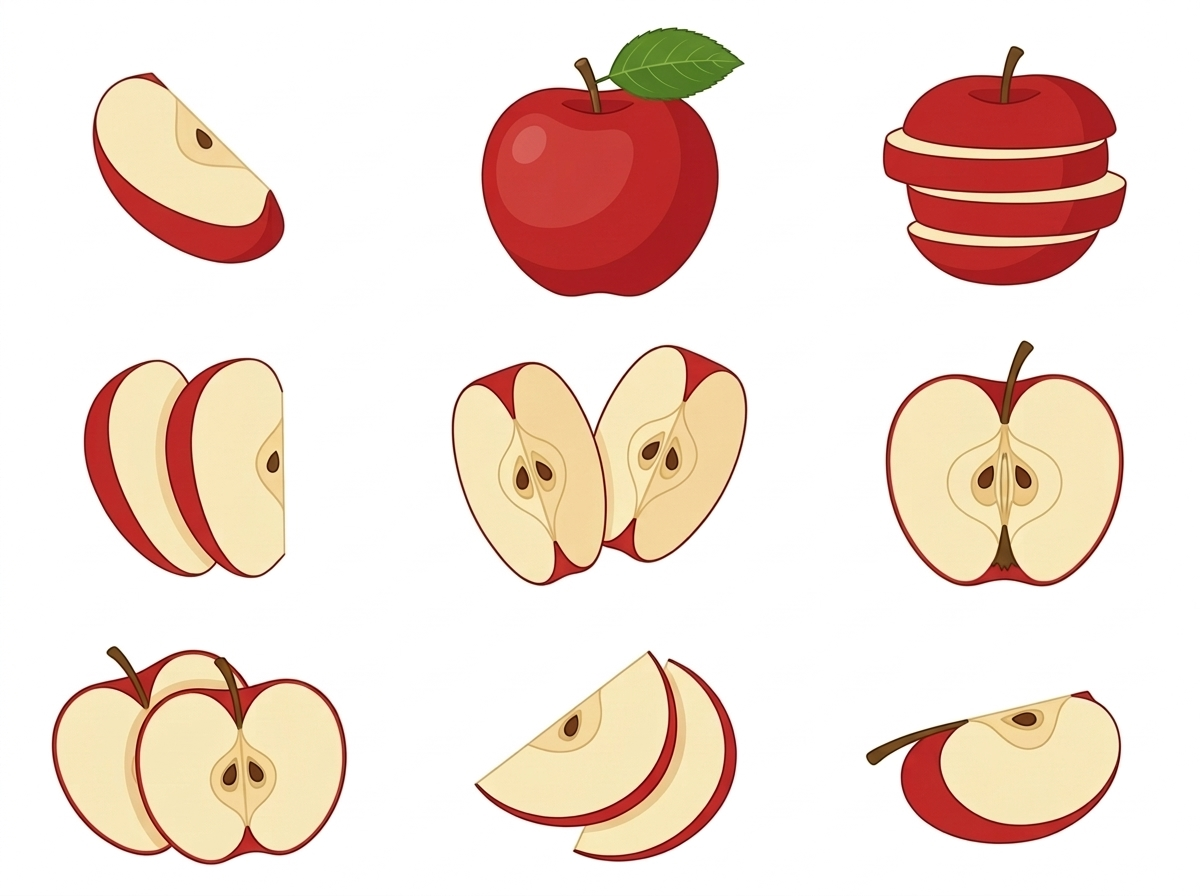
\includegraphics[width=0.45\textwidth]{figures/apple.png}
	\captionof{figure}[附录 B 中补充图片占位示例]{附录 B 中补充图片占位示例。\par
		（A）XXXX；（B）XXXX；（C）XXXX。\par
		注：不同小写字母代表存在显著差异（$p<0.05$）。\par
		{\qauTimes\fontsize{10.5bp}{15.75bp}\selectfont \textbf{Fig.~\thefigure\ Example of supplementary figure in Appendix B.}}\par
		{\qauTimes\fontsize{10.5bp}{15.75bp}\selectfont \textbf{(A) XXXX; (B) XXXX; (C) XXXX.}}\par
        {\qauTimes\fontsize{10.5bp}{15.75bp}\selectfont \textbf{Different lowercase letters indicate significant differences (\boldmath$p<0.05$).}}}
	\label{fig:appendix-b-figure}
\end{center}
\QAUbackmattertitle{导师组意见}%
{{\QAUkaiTitle\bfseries\fontsize{16bp}{48bp}\selectfont 导师组意见}}%
\label{chap:opinion}

{\kaishu\fontsize{14bp}{21bp}\selectfont
	导师组已通过\QAUcoverlineKai[2.8cm]{\qauauthor}的论文审查，同意并推荐其参加硕士学位论文答辩。\par}

\vspace{5.8cm}

{\kaishu\zihao{4}\noindent\hspace*{8.2cm}导\hspace{2.2em}师：\par}

\vspace{1.25cm}

{\kaishu\zihao{4}\noindent\hspace*{8.2cm}导师组成员：\par}

\vspace{3.25cm}

\begin{flushright}
	\kaishu\zihao{4}年\hspace{2.8em}月\hspace{2.8em}日\hspace*{1.5cm}
\end{flushright}
\QAUchapterstar{致谢}\label{chap:acknowledgements}

\vspace{0.5\baselineskip}

时值论文完成之际，谨向在研究开展与论文撰写过程中给予指导、帮助和支持的老师、同学、亲友致以诚挚谢意。

XXXXXXX。

XXXXXXX。

XXXXXXX。
\QAUchapterstar{作者简历}\label{chap:resume}

\vspace{0.5\baselineskip}

{\songti\fontsize{12bp}{18bp}\selectfont
	
	\noindent\textbf{姓名：}张三\par
	
	\noindent\textbf{性别：}女\par
	
	\noindent\textbf{出生年月：}1999 年 6 月\par
	
	\noindent\textbf{籍贯：}山东青岛\par
	
	\noindent\textbf{教育经历：}
	\begin{enumerate}[leftmargin=3em,itemsep=0pt,topsep=5pt,partopsep=0pt,parsep=0pt]
		\item 2019 年 9 月--2023 年 6 月，青岛农业大学，食品科学与工程学院，食品科学与工程专业，本科。
		\item 2023 年 9 月--2026 年 6 月，青岛农业大学，食品科学与工程学院，食品科学与工程专业，硕士研究生。
	\end{enumerate}
	
	\noindent\textbf{研究方向：}鲜切果蔬品质控制\par
	
}
\QAUchapterstar{在读期间科研学术成果目录}\label{chap:achievements}

\vspace{0.5\baselineskip}

{\songti\fontsize{12bp}{18bp}\selectfont
	
	\begin{QAUitemblock}{一、发表论文}
		\item[1.] San Zhang，XXX XXX，XXX XXX. XXXXXXXXXXX[J]. \textit{Food Chemistry}, 2026, XXX: XXXXXX.
		\item[2.] San Zhang，XXX XXX，XXX XXX. XXXXXXXXXXX[J]. \textit{Food Control}, 2026, XXX: XXXXXX.
		\item[3.] San Zhang，XXX XXX，XXX XXX. XXXXXXXXXXX[J]. \textit{Food Hydrocolloids}, 2026, XXX: XXXXXX.
	\end{QAUitemblock}
	
	\begin{QAUitemblock}{二、专利与软件著作权}
		\item[1.] 张三，李四. 一种用于鲜切果蔬护色处理的浸渍方法[P]. 中国发明专利，申请号：202610000001.X。
	\end{QAUitemblock}
	
}

\end{document}
